\let\negmedspace\undefined
\let\negthickspace\undefined
\documentclass[journal]{IEEEtran}
\usepackage[a5paper, margin=10mm, onecolumn]{geometry}
\usepackage{tfrupee} 

\setlength{\headheight}{1cm} 
\setlength{\headsep}{0mm}  
\usepackage{gvv-book}
\usepackage{gvv}

\usepackage{cite}
\usepackage{amsmath,amssymb,amsfonts,amsthm}
\usepackage{algorithmic}
\usepackage{graphicx}
\usepackage{textcomp}
\usepackage{xcolor}
\usepackage{txfonts}
\usepackage{listings}
\usepackage{enumitem}
\usepackage{mathtools}
\usepackage{gensymb}
\usepackage{comment}
\usepackage[breaklinks=true]{hyperref}
\usepackage{tkz-euclide} 
\usepackage{listings}
% \usepackage{gvv}                                        
\def\inputGnumericTable{}                                 
\usepackage[latin1]{inputenc}                                
\usepackage{color}                                            
\usepackage{array}                                            
\usepackage{longtable}                                       
\usepackage{calc}                                             
\usepackage{multirow}                                         
\usepackage{hhline}                                           
\usepackage{ifthen}                                           
\usepackage{lscape}
\usepackage{tikz}
\usetikzlibrary{patterns}
\begin{document}

\bibliographystyle{IEEEtran}
\vspace{3cm}


\title{GATE 2009 ME }
\author{ee25btech11029- Jnanesh Sathisha Karmar}
\maketitle
% \maketitle
% \newpage
% \bigskip
{\let\newpage\relax\maketitle}

\renewcommand{\thefigure}{\theenumi}
\renewcommand{\thetable}{\theenumi}
\setlength{\intextsep}{10pt} % Space between text and floats
\begin{enumerate}[leftmargin=0pt]


\item
If $\rightarrow$ denotes increasing order of intensity, then the meaning of the words  \brak{\text{smile} \rightarrow \text{giggle} \rightarrow \text{laugh}} is analogous to \brak{\text{disapprove} \rightarrow \underline{\hspace{2cm}} \rightarrow \text{chide}}. 
Which one of the given options is appropriate to fill the blank?

\vspace{2mm}

\begin{enumerate}
\begin{multicols}{4}
\item reprove
\item praise
\item reprise
\item grieve
\end{multicols}
\end{enumerate}

\hfill{\brak{\text{GATE ME 2024}}}

\vspace{4mm}

\item
Find the odd one out in the set \brak{19, 37, 21, 17, 23, 29, 31, 11} 

\vspace{2mm}

\begin{enumerate}
\begin{multicols}{4}
\item 21 
\item 29 
\item 37 
\item 23
\end{multicols}
\end{enumerate}

\hfill{\brak{\text{GATE ME 2024}}}

\vspace{4mm}

\item
In the following series, identify the number that needs to be changed to form the Fibonacci series.
$1, 1, 2, 3, 6, 8, 13, 21,$ 

\vspace{2mm}

\begin{enumerate}
\begin{multicols}{4}
\item 8
\item 21
\item 6
\item 13
\end{multicols}
\end{enumerate}

\hfill{\brak{\text{GATE ME 2024}}}

\vspace{4mm}

\item
The real variables $x,y,z$, and the real constants $p,q,r$ satisfy 
\[
\frac{x}{pq - r^2} =
\frac{y}{qr - p^2} =
\frac{z}{rp - q^2}
\]
Given that the denominators are non-zero, the value of $px + qy + rz$ is 

\vspace{2mm}

\begin{enumerate}
\begin{multicols}{4}
\item 0
\item 1
\item $pqr$
\item $p^2 + q^2 + r^2$
\end{multicols}
\end{enumerate}

\hfill{\brak{\text{GATE ME 2024}}}

\vspace{4mm}

\item
Take two long dice \brak{\text{rectangular parallelepiped}}, each having four rectangular faces labelled as $2, 3, 5, 7$. If thrown, the long dice cannot land on the square faces and has $1/4$ probability of landing on any of the four rectangular faces. The label on the top face of the dice is the score of the throw. If thrown together, what is the probability of getting the sum of the two long dice scores greater than $11$?

\vspace{2mm}

\begin{enumerate}
\begin{multicols}{4}
\item $\frac{3}{8}$
\item $\frac{1}{8}$
\item $\frac{1}{16}$
\item $\frac{3}{16}$
\end{multicols}
\end{enumerate}

\hfill{\brak{\text{GATE ME 2024}}}


\item
In the given text, the blanks are numbered \brak{i}-\brak{iv}. Select the best match for all the blanks.  
Prof. P \brak{i} merely a man who narrated funny stories. \brak{ii} in his blackest moments he was capable of self-deprecating humor.  
Prof. Q \brak{iii} a man who hardly narrated funny stories. \brak{iv} in his blackest moments was he able to find humor.  

\vspace{2mm}

\begin{enumerate}
\begin{multicols}{4}
\item \brak{i} was, \brak{ii} Only, \brak{iii} wasn;t, \brak{iv} Even
\item \brak{i} wasn't, \brak{ii} Even, \brak{iii} was, \brak{iv} Only
\item \brak{i} was, \brak{ii} Even, \brak{iii} wasn't, \brak{iv} Only
\item \brak{i} wasn't, \brak{ii} Only, \brak{iii} was, \brak{iv} Even
\end{multicols}
\end{enumerate}

\hfill{\brak{\text{GATE ME 2024}}}

\vspace{4mm}

\item
How many combinations of non-null sets $A$, $B$, $C$ are possible from the subsets of \brak{2, 3, 5} satisfying the conditions: \brak{i} $A$ is a subset of $B$, and \brak{ii} $B$ is a subset of $C$?

\vspace{2mm}

\begin{enumerate}
\begin{multicols}{4}
\item 28
\item 27
\item 18
\item 19
\end{multicols}
\end{enumerate}

\hfill{\brak{\text{GATE ME 2024}}}

\vspace{4mm}

\item
The bar chart gives the batting averages of VK and RS for 11 calendar years from 2012 to 2022. Considering that 2015 and 2019 are world cup years, which one of the following options is true?
\begin{figure}[h]
\centering
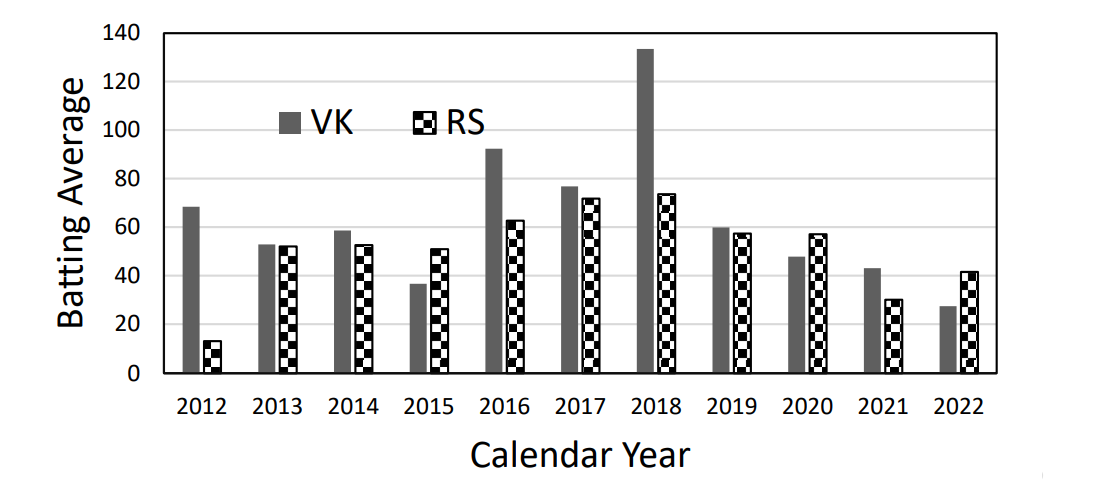
\includegraphics[width=0.5\columnwidth]{Figs/image (60).png}
\caption*{}
\label{fig:8}
\end{figure}

\vspace{2mm}

\begin{enumerate}

\item RS has a higher yearly batting average than that of VK in every world cup year.
\item VK has a higher yearly batting average than that of RS in every world cup year.
\item VK's yearly batting average is consistently higher than that of RS between the two world cup years.
\item RS,s yearly batting average is consistently higher than that of VK in the last three years.

\end{enumerate}

\hfill{\brak{\text{GATE ME 2024}}}

\vspace{4mm}

\item


A planar rectangular paper has two V-shaped pieces attached as shown above. 
\begin{figure}[h]
\centering
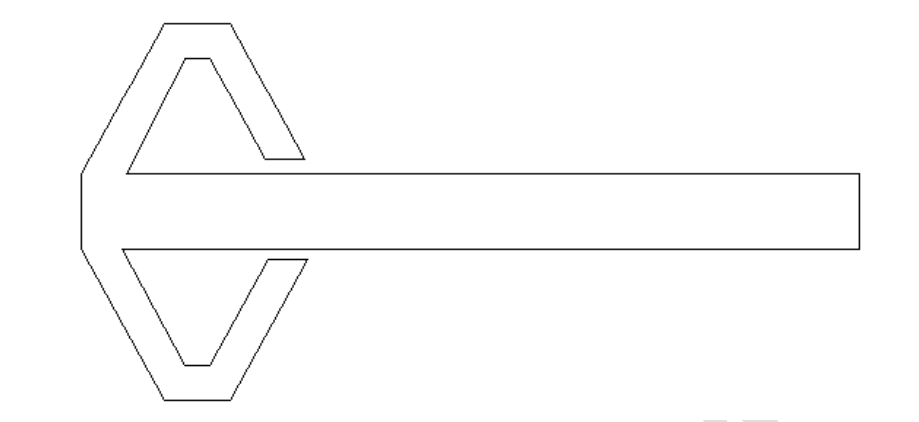
\includegraphics[width=0.5\columnwidth]{Figs/image (61).png}
\caption*{}
\label{fig:9}
\end{figure}
This piece of paper is folded to make the following closed three-dimensional object.
\begin{figure}[h]
\centering
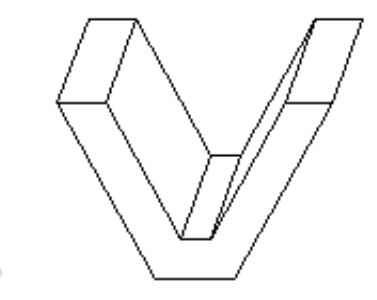
\includegraphics[width=0.3\columnwidth]{Figs/image (62).png}
\caption*{}
\label{fig:9}
\end{figure}

The number of folds required to form the above object is 

\vspace{2mm}

\begin{enumerate}
\begin{multicols}{4}
\item 9
\item 7
\item 11
\item 8
\end{multicols}
\end{enumerate}

\hfill{\brak{\text{GATE ME 2024}}}

\vspace{4mm}

\item
Four equilateral triangles are used to form a regular closed three-dimensional object by joining along the edges. The angle between any two faces is 

\vspace{2mm}

\begin{enumerate}
\begin{multicols}{4}
\item $30\degree$
\item $60\degree$
\item $45\degree$
\item $90\degree$
\end{multicols}
\end{enumerate}

\hfill{\brak{\text{GATE ME 2024}}}

\vspace{4mm}

\item
In order to numerically solve the ordinary differential equation
\[
\frac{dy}{dt} = -y \quad \text{for} \quad t > 0, \text{ with initial condition } y(0) = 1,
\]
the following scheme is employed
\[
\frac{y_{n+1} - y_n}{\Delta t} = -\frac{1}{2} \left(y_{n+1} + y_n \right).
\]
Here, $\Delta t$ is the time step and $y_n = y(n \Delta t)$ for $n = 0,1,2,\ldots$. This numerical scheme will yield a solution with non-physical oscillations for $\Delta t > h$. The value of $h$ is

\vspace{2mm}

\begin{enumerate}
\begin{multicols}{4}
\item $\frac{1}{2}$
\item $1$
\item $\frac{3}{2}$
\item $2$
\end{multicols}
\end{enumerate}

\hfill{\brak{\text{GATE ME 2024}}}

\vspace{4mm}

\item
The value of the surface integral
\[
\oint_S z \, dx \, dy,
\]
where $S$ is the external surface of the sphere $x^2 + y^2 + z^2 = R^2$ is

\vspace{2mm}

\begin{enumerate}
\begin{multicols}{4}
\item $0$
\item $4 \pi R^3$
\item $\frac{4 \pi}{3} R^3$
\item $\pi R^3$
\end{multicols}
\end{enumerate}

\hfill{\brak{\text{GATE ME 2024}}}

\vspace{4mm}

\item
Let $f(z)$ be an analytic function, where $z = x + iy$. If the real part of $f(z)$ is $\cosh x \cos y$, and the imaginary part of $f(z)$ is zero for $y=0$, then $f(z)$ is

\vspace{2mm}

\begin{enumerate}
\begin{multicols}{4}
\item $\cosh x \exp(-iy)$
\item $\cosh z \exp z$
\item $\cosh z \cos y$
\item $\cosh z$
\end{multicols}
\end{enumerate}

\hfill{\brak{\text{GATE ME 2024}}}

\vspace{4mm}

\item
Consider the system of linear equations
\begin{align*}
x + 2y + z &= 5 \\
2x + a y + 4z &= 12 \\
2x + 4y + 6z &= b
\end{align*}

The values of $a$ and $b$ such that there exists a non-trivial null space and the system admits infinite solutions are

\vspace{2mm}

\begin{enumerate}
\begin{multicols}{4}
\item $a=8, b=14$
\item $a=4, b=12$
\item $a=8, b=12$
\item $a=4, b=14$
\end{multicols}
\end{enumerate}

\hfill{\brak{\text{GATE ME 2024}}}

\vspace{4mm}

\item
Let $f(\cdot)$ be a twice differentiable function from $\mathbb{R}^2 \to \mathbb{R}$. If $\myvec{p}, \myvec{x_0} \in \mathbb{R}^2$ where $\abs{p}$ is sufficiently small (here $\abs{\cdot}$ is the Euclidean norm), then
\[
f(\myvec{x_0} + \myvec{p}) = f(\myvec{x_0}) + \nabla f(\myvec{x_0})^T \myvec{p} + \frac{1}{2} \myvec{p}^T \nabla^2 f(\psi) \myvec{p}
\]
where $\psi \in \mathbb{R}^2$ is a point on the line segment joining $\myvec{x_0}$ and $\myvec{x_0} + \myvec{p}$. If $\myvec{x_0}$ is a strict local minimum of $f(\myvec{x})$, then which one of the following statements is TRUE?

\vspace{2mm}

\begin{enumerate}
\begin{multicols}{4}
\item $\nabla f(\myvec{x_0})^T \myvec{p} > 0$ and $\myvec{p}^T \nabla^2 f(\psi) \myvec{p} = 0$
\item $\nabla f(\myvec{x_0})^T \myvec{p} = 0$ and $\myvec{p}^T \nabla^2 f(\psi) \myvec{p} > 0$
\item $\nabla f(\myvec{x_0})^T \myvec{p} = 0$ and $\myvec{p}^T \nabla^2 f(\psi) \myvec{p} = 0$
\item $\nabla f(\myvec{x_0})^T \myvec{p} = 0$ and $\myvec{p}^T \nabla^2 f(\psi) \myvec{p} < 0$
\end{multicols}
\end{enumerate}

\hfill{\brak{\text{GATE ME 2024}}}

\vspace{4mm}

\item
The velocity field of a two-dimensional, incompressible flow is given by
\[
\myvec{V} = 2 \sinh x \, \hat{i} + v(x,y) \, \hat{j}
\]
where $\hat{i}$ and $\hat{j}$ denote the unit vectors in $x$ and $y$ directions, respectively. If $v(x,0) = \cosh x$, then $v(0,-1)$ is

\vspace{2mm}

\begin{enumerate}
\begin{multicols}{4}
\item $1$
\item $2$
\item $3$
\item $4$
\end{multicols}
\end{enumerate}

\hfill{\brak{\text{GATE ME 2024}}}

\item
A plane, solid slab of thickness $L$, shown in the figure, has thermal conductivity $k$ that varies with the spatial coordinate $x$ as $k = A + Bx$, where $A$ and $B$ are positive constants $\brak{A > 0, B > 0}$. The slab walls are maintained at fixed temperatures of $T\brak{x = 0} = 0$ and $T\brak{x = L} = T_0 > 0$. The slab has no internal heat sources. Considering one-dimensional heat transfer, which one of the following plots qualitatively depicts the steady-state temperature distribution within the slab?

\begin{figure}[h]
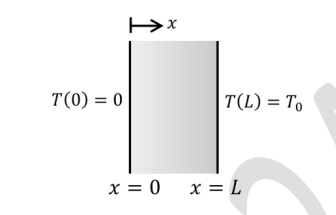
\includegraphics[width=0.40\columnwidth]{Figs/image (63).png}
\caption*{}
\label{fig:17}
\end{figure}

\vspace{2mm}
\begin{enumerate}
\item
\begin{figure}[h]
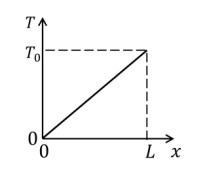
\includegraphics[width=0.24\columnwidth]{Figs/image (64).png}
\caption*{}
\label{fig:a}
\end{figure}
\item
\begin{figure}[h]
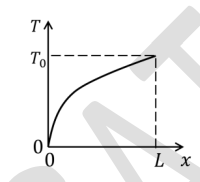
\includegraphics[width=0.24\columnwidth]{Figs/image (65).png}
\caption*{}
\label{fig:b}
\end{figure}
\item
\begin{figure}[h]
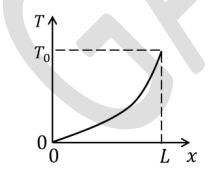
\includegraphics[width=0.24\columnwidth]{Figs/image (66).png}
\caption*{}
\label{fig:c}
\end{figure}
\item
\begin{figure}[h]
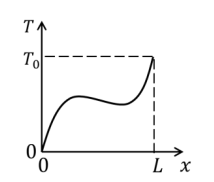
\includegraphics[width=0.24\columnwidth]{Figs/image (67).png}
\caption*{}
\label{fig:d}
\end{figure}
\end{enumerate}

\hfill{\brak{\text{GATE ME 2024}}}

\vspace{4mm}

\item
Consider incompressible laminar flow over a flat plate with freestream velocity of $u_\infty$. The Nusselt number corresponding to this flow velocity is $Nu_1$. If the freestream velocity is doubled, the Nusselt number changes to $Nu_2$. Choose the correct option for $\frac{Nu_2}{Nu_1}$.

\vspace{2mm}

\begin{enumerate}
\begin{multicols}{4}
\item $\sqrt{2}$
\item $2$
\item $1.26$
\item $1$
\end{multicols}
\end{enumerate}

\hfill{\brak{\text{GATE ME 2024}}}

\vspace{4mm}

\item
Consider a hydrodynamically fully developed laminar flow through a circular pipe with the flow along the axis \brak{i.e., z direction}. In the following statements, $T$ is the temperature of the fluid, $T_w$ is the wall temperature and $T_m$ is the bulk mean temperature of the fluid. Which one of the following statements is TRUE?

\vspace{2mm}

\begin{enumerate}
\begin{multicols}{4}
\item For a thermally fully developed flow, $\frac{\partial T}{\partial z} = 0$, always.
\item For constant wall temperature of the duct, $\frac{dT_m}{dz} = \text{constant}$.
\item Nusselt number varies linearly along the $z$ direction for a thermally fully developed flow.
\item For constant wall temperature $\brak{T_w > T_m}$ of the duct, $\frac{dT_m}{dz}$ increases exponentially with distance along $z$ direction.
\end{multicols}
\end{enumerate}

\hfill{\brak{\text{GATE ME 2024}}}

\vspace{4mm}

\item
A furnace can supply heat steadily at $1200\text{K}$ at a rate of $24000~\text{kJ/min}$. The maximum amount of power $\brak{\text{in kW}}$ that can be produced by using the heat supplied by this furnace in an environment at $300\text{K}$ is

\vspace{2mm}

\begin{enumerate}
\begin{multicols}{4}
\item $300$
\item $150$
\item $18000$
\item $0$
\end{multicols}
\end{enumerate}

\hfill{\brak{\text{GATE ME 2024}}}

\vspace{4mm}

\item
Which one of the following statements regarding a Rankine cycle is FALSE?

\vspace{2mm}

\begin{enumerate}
\begin{multicols}{4}
\item Superheating the steam in the boiler increases the cycle efficiency.
\item The pressure at the turbine outlet depends on the condenser temperature.
\item Cycle efficiency increases as condenser pressure decreases.
\item Cycle efficiency increases as boiler pressure decreases.
\end{multicols}
\end{enumerate}

\hfill{\brak{\text{GATE ME 2024}}}

\vspace{4mm}

\item
For a ball bearing, the fatigue life in millions of revolutions is given by $L = \left(\frac{C}{P}\right)^n$, where $P$ is the constant applied load and $C$ is the basic dynamic load rating. Which one of the following statements is TRUE?

\vspace{2mm}

\begin{enumerate}
\begin{multicols}{4}
\item $n = 3$, assuming that the inner racing is fixed and outer racing is revolving
\item $n = \frac{1}{3}$, assuming that the inner racing is fixed and outer racing is revolving
\item $n = 3$, assuming that the outer racing is fixed and inner racing is revolving
\item $n = \frac{1}{3}$, assuming that the outer racing is fixed and inner racing is revolving
\end{multicols}
\end{enumerate}

\hfill{\brak{\text{GATE ME 2024}}}

\vspace{4mm}

\item
The change in kinetic energy $\Delta E$ of an engine is $300~\text{J}$, and minimum and maximum shaft speeds are $\omega_{min} = 220~\text{rad/s}$ and $\omega_{max} = 280~\text{rad/s}$, respectively. Assume that the torque-time function is purely harmonic. To achieve a coefficient of fluctuation of $0.05$, the moment of inertia $\brak{\text{in kg.m}^2}$ of the flywheel to be mounted on the engine shaft is

\vspace{2mm}

\begin{enumerate}
\begin{multicols}{4}
\item $0.113$
\item $0.096$
\item $0.071$
\item $0.053$
\end{multicols}
\end{enumerate}

\hfill{\brak{\text{GATE ME 2024}}}

\item
A ram in the form of a rectangular body of size $l = 9~\text{m}$ and $b = 2~\text{m}$ is suspended by two parallel ropes of lengths $7~\text{m}$. Assume the center-of-mass of the body is at its geometric center and $g = 9.81~\text{m/s}^2$. For striking the object P with a horizontal velocity of $5~\text{m/s}$, what is the angle $\theta$ with the vertical from which the ram should be released from rest?

\begin{figure}[h]
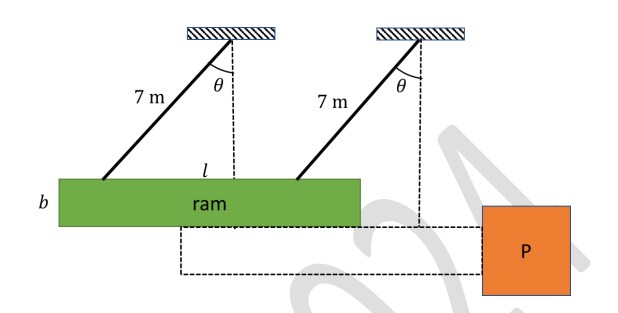
\includegraphics[width=0.6\columnwidth]{Figs/image (68).png}
\caption*{}
\label{fig:q24}
\end{figure}

\vspace{2mm}

\begin{enumerate}
\begin{multicols}{4}
\item $67.1\degree$
\item $40.2\degree$
\item $35.1\degree$
\item $79.5\degree$
\end{multicols}
\end{enumerate}

\hfill{\brak{\text{GATE ME 2024}}}

\vspace{4mm}

\item
A linear spring-mass-dashpot system with a mass of $2~\text{kg}$ is set in motion with viscous damping. If the natural frequency is $15~\text{Hz}$, and the amplitudes of two successive cycles measured are $7.75~\text{mm}$ and $7.20~\text{mm}$, the coefficient of viscous damping $\brak{\text{in N.s/m}}$ is

\vspace{2mm}

\begin{enumerate}
\begin{multicols}{4}
\item $4.41$
\item $7.51$
\item $2.52$
\item $6.11$
\end{multicols}
\end{enumerate}

\hfill{\brak{\text{GATE ME 2024}}}

\vspace{4mm}

\item
Which one of the following failure theories is the most conservative design approach against fatigue failure?

\vspace{2mm}

\begin{enumerate}
\begin{multicols}{2}
\item Soderberg line
\item Modified Goodman line
\item Gerber line
\item Yield line
\end{multicols}
\end{enumerate}

\hfill{\brak{\text{GATE ME 2024}}}

\vspace{4mm}

\item
A rigid massless tetrahedron is placed such that vertex O is at the origin and the other three vertices A, B, and C lie on the coordinate axes as shown in the figure. The body is acted on by three point loads, of which one is acting at A along $x$-axis and another at point B along $y$-axis. For the body to be in equilibrium, the third point load acting at point O must be

\begin{figure}[h]
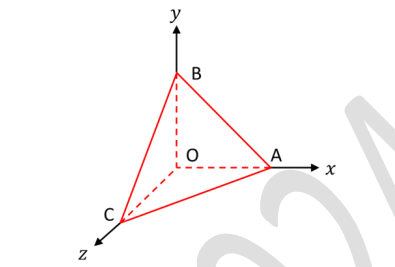
\includegraphics[width=0.45\columnwidth]{Figs/image (69).png}
\caption*{}
\label{fig:q27}
\end{figure}

\vspace{2mm}

\begin{enumerate}
\begin{multicols}{4}
\item along $z$-axis
\item in $x$-$y$ plane but not along $x$ or $y$ axis
\item in $y$-$z$ plane but not along $y$ or $z$ axis
\item in $z$-$x$ plane but not along $z$ or $x$ axis
\end{multicols}
\end{enumerate}

\hfill{\brak{\text{GATE ME 2024}}}

\vspace{4mm}

\item
The phases present in pearlite are

\vspace{2mm}

\begin{enumerate}
\begin{multicols}{4}
\item austenite and ferrite
\item cementite and austenite
\item ferrite and cementite
\item martensite and ferrite
\end{multicols}
\end{enumerate}

\hfill{\brak{\text{GATE ME 2024}}}

\vspace{4mm}

\item
The "Earing" phenomenon in metal forming is associated with

\vspace{2mm}

\begin{enumerate}
\begin{multicols}{4}
\item deep drawing
\item rolling
\item extrusion
\item forging
\end{multicols}
\end{enumerate}

\hfill{\brak{\text{GATE ME 2024}}}

\vspace{4mm}

\item
The grinding wheel used to provide the best surface finish is

\vspace{2mm}

\begin{enumerate}
\begin{multicols}{4}
\item A36L5V
\item A54L5V
\item A60L5V
\item A80L5V
\end{multicols}
\end{enumerate}

\hfill{\brak{\text{GATE ME 2024}}}

\item
The allowance provided to a pattern for easy withdrawal from a sand mold is

\vspace{2mm}

\begin{enumerate}
\begin{multicols}{4}
\item finishing allowance
\item shrinkage allowance
\item distortion allowance
\item shake allowance
\end{multicols}
\end{enumerate}

\hfill{\brak{\text{GATE ME 2024}}}

\vspace{4mm}

\item
The most suitable electrode material used for joining low alloy steels using Gas Metal Arc Welding (GMAW) process is

\vspace{2mm}

\begin{enumerate}
\begin{multicols}{4}
\item copper
\item cadmium
\item low alloy steel
\item tungsten
\end{multicols}
\end{enumerate}

\hfill{\brak{\text{GATE ME 2024}}}

\vspace{4mm}

\item
The preparatory functions in Computer Numerical Controlled (CNC) machine programing are denoted by the alphabet

\vspace{2mm}

\begin{enumerate}
\begin{multicols}{4}
\item G
\item M
\item P
\item O
\end{multicols}
\end{enumerate}

\hfill{\brak{\text{GATE ME 2024}}}

\vspace{4mm}

\item
A set of jobs $U, V, W, X, Y, Z$ arrive at time $t = 0$ to a production line consisting of two workstations in series. Each job must be processed by both workstations in sequence \brak{\text{i.e., the first followed by the second}}. The process times \brak{\text{in minutes}} for each job on each workstation in the production line are given below.

\begin{table}[h]
\centering
\begin{tabular}{|l|c|c|c|c|c|c|} \hline
Job           & U & V & W & X & Y & Z \\ \hline
Workstation 1 & 5 & 7 & 3 & 4 & 6 & 8 \\ \hline
Workstation 2 & 4 & 6 & 6 & 8 & 5 & 7 \\ \hline
\end{tabular}
\caption*{}
\label{tab:Q34}
\end{table}

The sequence in which the jobs must be processed by the production line if the total makespan of production is to be minimized is

\vspace{2mm}

\begin{enumerate}
\begin{multicols}{4}
\item W-X-Z-V-Y-U
\item W-X-V-Z-Y-U
\item W-U-Z-V-Y-X
\item U-Y-V-Z-X-W
\end{multicols}
\end{enumerate}

\hfill{\brak{\text{GATE ME 2024}}}

\vspace{4mm}

\item
A queueing system has one single server workstation that admits an infinitely long queue. The rate of arrival of jobs to the queueing system follows the Poisson distribution with a mean of $5$ jobs/hour. The service time of the server is exponentially distributed with a mean of $6$ minutes. In steady state operation of the queueing system, the probability that the server is not busy at any point in time is

\vspace{2mm}

\begin{enumerate}
\begin{multicols}{4}
\item $0.20$
\item $0.17$
\item $0.50$
\item $0.83$
\end{multicols}
\end{enumerate}

\hfill{\brak{\text{GATE ME 2024}}}

\vspace{4mm}

\item
The matrix $\myvec{1 & a \\ 8 & 3}$ (where $a > 0$) has a negative eigenvalue if $a$ is greater than

\vspace{2mm}

\begin{enumerate}
\begin{multicols}{4}
\item $\frac{3}{8}$
\item $\frac{1}{8}$
\item $\frac{1}{4}$
\item $\frac{1}{5}$
\end{multicols}
\end{enumerate}

\hfill{\brak{\text{GATE ME 2024}}}



\item
In the pipe network shown in the figure, all pipes have the same cross-section and can be assumed to have the same friction factor. The pipes connecting points $W$, $N$, and $S$ with point $J$ have an equal length $L$. The pipe connecting points $J$ and $E$ has a length $10L$. The pressures at the ends $N$, $E$, and $S$ are equal. The flow rate in the pipe connecting $W$ and $J$ is $Q$. Assume that the fluid flow is steady, incompressible, and the pressure losses at the pipe entrance and junction are negligible. Consider the following statements:

I : The flow rate in pipe connecting $J$ and $E$ is $Q/21$.\\
II : The pressure difference between $J$ and $N$ is equal to the pressure difference between $J$ and $E$.

Which one of the following options is CORRECT?

\begin{figure}[h]
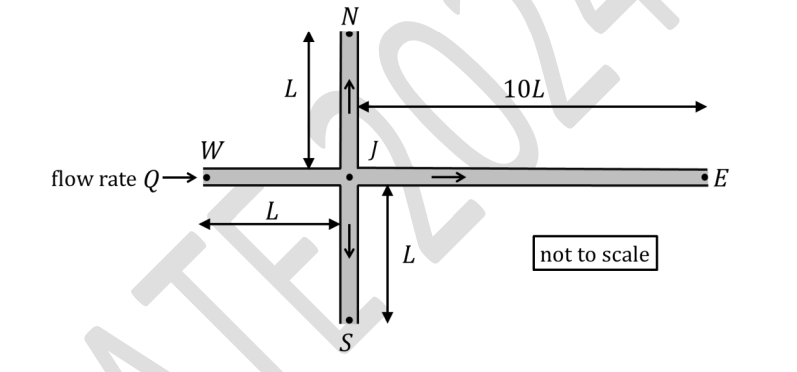
\includegraphics[width=0.55\columnwidth]{Figs/image (70).png}
\caption*{}
\label{fig:q37}
\end{figure}

\vspace{2mm}

\begin{enumerate}
\begin{multicols}{2}
\item I is True and II is False
\item I is False and II is True
\item Both I and II are True
\item Both I and II are False
\end{multicols}
\end{enumerate}

\hfill{\brak{\text{GATE ME 2024}}}

\vspace{4mm}

\item
A company orders gears in conditions identical to those considered in the economic order quantity \brak{EOQ} model in inventory control. The annual demand is $8000$ gears, the cost per order is $300$ rupees, and the holding cost is $12$ rupees per month per gear. The company uses an order size that is $25\%$ more than the optimal order quantity determined by the EOQ model. The percentage change in the total cost of ordering and holding inventory from that associated with the optimal order quantity is

\vspace{2mm}

\begin{enumerate}
\begin{multicols}{4}
\item $2.5$
\item $5$
\item $0$
\item $12.5$
\end{multicols}
\end{enumerate}

\hfill{\brak{\text{GATE ME 2024}}}

\vspace{4mm}

\item
At the current basic feasible solution (bfs) $\myvec{v_0} \brak{\myvec{v_0} \in \mathbb{R}^5}$, the simplex method yields the following form of a linear programming problem in standard form.
\begin{align*}
\text{minimize} \quad &z = -x_1 - 2x_2 \\
\text{s.t.}\quad\quad
&x_3 = 2 + 2x_1 - x_2 \\
&x_4 = 7 + x_1 - 2x_2 \\
&x_5 = 3 - x_1 \\
&\text{x}_1,\ \text{x}_2,\ \text{x}_3,\ \text{x}_4,\ \text{x}_5 \geq 0
\end{align*}
Here the objective function is written as a function of the non-basic variables. If the simplex method moves to the adjacent bfs $\myvec{v_1} \brak{\myvec{v_1} \in \mathbb{R}^5}$ that best improves the objective function, which of the following represents the objective function at $\myvec{v_1}$, assuming that the objective function is written in the same manner as above?

\vspace{2mm}

\begin{enumerate}
\begin{multicols}{2}
\item $z = -4 - 5x_1 + 2x_3$
\item $z = -3 + x_5 - 2x_2$
\item $z = -4 - 5x_1 + 2x_4$
\item $z = -6 - 5x_1 + 2x_3$
\end{multicols}
\end{enumerate}

\hfill{\brak{\text{GATE ME 2024}}}

\vspace{4mm}

\item
Steady, compressible flow of air takes place through an adiabatic converging-diverging nozzle, as shown in the figure. For a particular value of pressure difference across the nozzle, a stationary normal shock wave forms in the diverging section of the nozzle. If $E$ and $F$ denote the flow conditions just upstream and downstream of the normal shock, respectively, which of the following statement(s) is/are TRUE?

\begin{figure}[h]
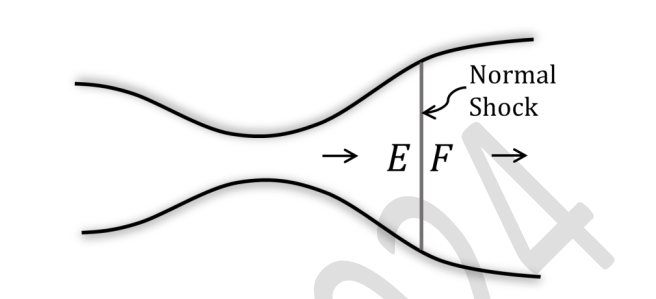
\includegraphics[width=0.45\columnwidth]{Figs/image (71).png}
\caption*{}
\label{fig:q40}
\end{figure}

\vspace{2mm}

\begin{enumerate}
\begin{multicols}{2}
\item Static pressure at $E$ is lower than the static pressure at $F$
\item Density at $E$ is lower than the density at $F$
\item Mach number at $E$ is lower than the Mach number at $F$
\item Specific entropy at $E$ is lower than the specific entropy at $F$
\end{multicols}
\end{enumerate}

\hfill{\brak{\text{GATE ME 2024}}}

\vspace{4mm}

\item
Which of the following beam(s) is/are statically indeterminate?

\vspace{2mm}

\begin{enumerate}
\item
\begin{figure}[h]
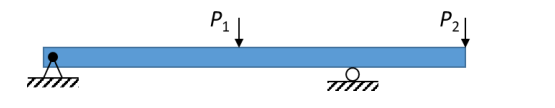
\includegraphics[width=0.42\columnwidth]{Figs/image (72).png}
\caption*{}
\label{fig:a}
\end{figure}
\item
\begin{figure}[h]
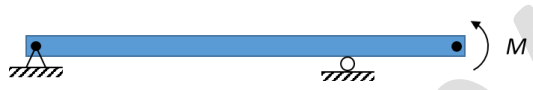
\includegraphics[width=0.42\columnwidth]{Figs/image (73).png}
\caption*{}
\label{fig:b}
\end{figure}
\item
\begin{figure}[h]
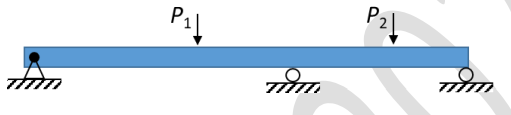
\includegraphics[width=0.42\columnwidth]{Figs/image (74).png}
\caption*{}
\label{fig:c}
\end{figure}
\item
\begin{figure}[h]
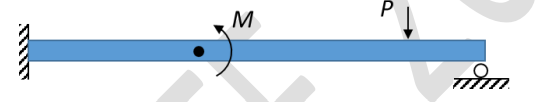
\includegraphics[width=0.42\columnwidth]{Figs/image (75).png}
\caption*{}
\label{fig:d}
\end{figure}
\end{enumerate}

\hfill{\brak{\text{GATE ME 2024}}}

\vspace{4mm}

\item
If the value of the double integral
\[
\int_{x=3}^{4}\int_{y=1}^{2}\frac{dy\,dx}{\brak{x+y}^2}
\]
is $\log_e\brak{a/24}$, then $a$ is \underline{\hspace{2cm}} \brak{\text{answer in integer}}.

\hfill{\brak{\text{GATE ME 2024}}}

\vspace{4mm}

\item
If $x\brak{t}$ satisfies the differential equation
\[
t\frac{dx}{dt} + \brak{t - x} = 0
\]
subject to the condition $x\brak{1} = 0$, then the value of $x\brak{2}$ is \underline{\hspace{2cm}} \brak{\text{rounded off to 2 decimal places}}.

\hfill{\brak{\text{GATE ME 2024}}}

\item
Let $X$ be a continuous random variable defined on $[0, 1]$ such that its probability density function $f(x) = 1$ for $0 \leq x \leq 1$ and $0$ otherwise. Let $Y = \log_e \brak{X + 1}$. Then the expected value of $Y$ is \underline{\hspace{2cm}} \brak{\text{rounded off to 2 decimal places}}.

\hfill{\brak{\text{GATE ME 2024}}}

\vspace{4mm}

\item
Consider an air-standard Brayton cycle with adiabatic compressor and turbine, and a regenerator, as shown in the figure. Air enters the compressor at $100~\text{kPa}$ and $300~\text{K}$ and exits the compressor at $600~\text{kPa}$ and $550~\text{K}$. The air exits the combustion chamber at $1250~\text{K}$ and exits the adiabatic turbine at $100~\text{kPa}$ and $800~\text{K}$. The exhaust air from the turbine is used to preheat the air in the regenerator. The exhaust air exits the regenerator (state 6) at $600~\text{K}$. There is no pressure drop across the regenerator and the combustion chamber. Also, there is no heat loss from the regenerator to the surroundings. The ratio of specific heats at constant pressure and volume is $c_p/c_v = 1.4$. The thermal efficiency of the cycle is \underline{\hspace{2cm}}\,\% \brak{\text{answer in integer}}.

\begin{figure}[h]
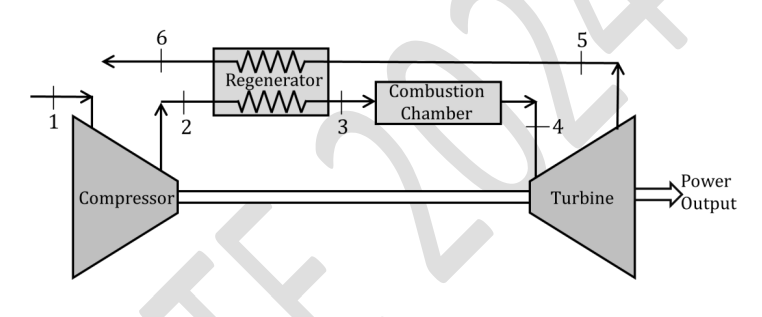
\includegraphics[width=0.6\columnwidth]{Figs/image (76).png}
\caption*{}
\label{fig:q45}
\end{figure}

\hfill{\brak{\text{GATE ME 2024}}}

\vspace{4mm}

\item
A piston-cylinder arrangement shown in the figure has a stop located $2~\text{m}$ above the base. The cylinder initially contains air at $140~\text{kPa}$ and $350~\degree$C and the piston is resting in equilibrium at a position which is $1~\text{m}$ above the stops. The system is now cooled to the ambient temperature of $25~\degree$C. Consider air to be an ideal gas with a value of gas constant $R = 0.287~\text{kJ}/(\text{kg}\cdot\text{K})$. The absolute value of specific work done during the process is \underline{\hspace{2cm}}~kJ/kg \brak{\text{rounded off to 1 decimal place}}.

\begin{figure}[h]
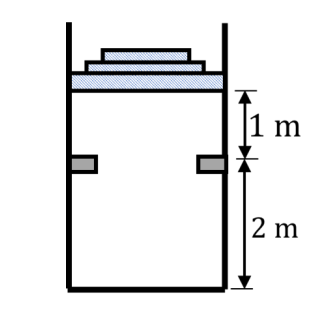
\includegraphics[width=0.33\columnwidth]{Figs/image (77).png}
\caption*{}
\label{fig:q46}
\end{figure}
\newpage

\hfill{\brak{\text{GATE ME 2024}}}

\vspace{4mm}

\item
A heat pump (H.P.) is driven by the work output of a heat engine (H.E.) as shown in the figure. The heat engine extracts $150~\text{kJ}$ of heat from the source at $1000~\text{K}$. The heat pump absorbs heat from the ambient at $280~\text{K}$ and delivers heat to the room which is maintained at $300~\text{K}$. Considering the combined system to be ideal, the total amount of heat delivered to the room together by the heat engine and heat pump is \underline{\hspace{2cm}}~kJ \brak{\text{answer in integer}}.

\begin{figure}[h]
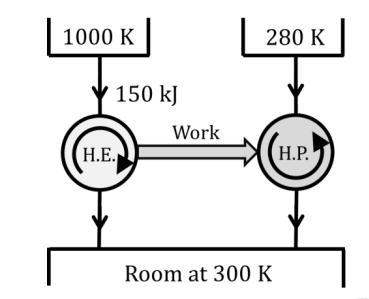
\includegraphics[width=0.47\columnwidth]{Figs/image (78).png}
\caption*{}
\label{fig:q47}
\end{figure}

\hfill{\brak{\text{GATE ME 2024}}}

\vspace{4mm}

\item
Consider a slab of $20~\text{mm}$ thickness. There is a uniform heat generation of $\dot{q} = 100~\text{MW}/\text{m}^3$ inside the slab. The left and right faces of the slab are maintained at $150~\degree$C and $110~\degree$C, respectively. The plate has a constant thermal conductivity of $200~\text{W}/(\text{m}\cdot\text{K})$. Considering a 1-D steady state heat conduction, the location of the maximum temperature from the left face will be at \underline{\hspace{2cm}}~mm \brak{\text{answer in integer}}.

\begin{figure}[h]
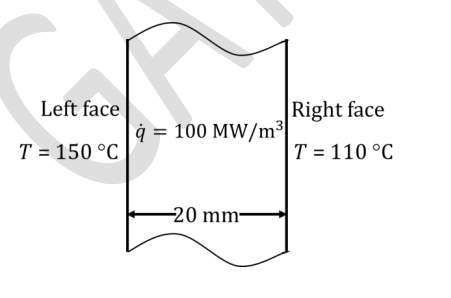
\includegraphics[width=0.36\columnwidth]{Figs/image (79).png}
\caption*{}
\label{fig:q48}
\end{figure}

\hfill{\brak{\text{GATE ME 2024}}}

\vspace{4mm}

\item
A condenser is used as a heat exchanger in a large steam power plant in which steam is condensed to liquid water. The condenser is a shell and tube heat exchanger which consists of $1$ shell and $20,000$ tubes. Water flows through each of the tubes at a rate of $1~\text{kg/s}$ with an inlet temperature of $30~\degree$C. The steam in the condenser shell condenses at the rate of $430~\text{kg/s}$ at a temperature of $50~\degree$C. If the heat of vaporization is $2.326~\text{MJ/kg}$ and specific heat of water is $4~\text{kJ}/(\text{kg}\cdot\text{K})$, the effectiveness of the heat exchanger is \underline{\hspace{2cm}} \brak{\text{rounded off to 3 decimal places}}.

\hfill{\brak{\text{GATE ME 2024}}}

\vspace{4mm}

\item
Consider a hemispherical furnace of diameter $D = 6~\text{m}$ with a flat base. The dome of the furnace has emissivity of $0.7$ and the flat base is a blackbody. The base and the dome are maintained at uniform temperature of $300~\text{K}$ and $1200~\text{K}$, respectively. Under steady state conditions, the rate of radiation heat transfer from the dome to the base is \underline{\hspace{2cm}}~kW \brak{\text{rounded off to the nearest integer}}.

Use Stefan-Boltzmann constant $= 5.67 \times 10^{-8}\,\text{W}/(\text{m}^2\,\text{K}^4)$.

\begin{figure}[h]
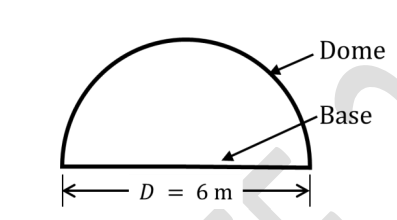
\includegraphics[width=0.44\columnwidth]{Figs/image (80).png}
\caption*{}
\label{fig:q50}
\end{figure}

\hfill{\brak{\text{GATE ME 2024}}}

\vspace{4mm}

\item
A liquid fills a horizontal capillary tube whose one end is dipped in a large pool of the liquid. Experiments show that the distance $L$ travelled by the liquid meniscus inside the capillary in time $t$ is given by
\[
L = k \gamma^a R^b \mu^c \sqrt{t}
\]
where $\gamma$ is the surface tension, $R$ is the inner radius of the capillary, and $\mu$ is the dynamic viscosity of the liquid. If $k$ is a dimensionless constant, then the exponent $a$ is \underline{\hspace{2cm}} \brak{\text{rounded off to 1 decimal place}}.

\hfill{\brak{\text{GATE ME 2024}}}

\vspace{4mm}

\item
The Levai type-A train illustrated in the figure has gears with module $m = 8~\text{mm/tooth}$. Gears 2 and 3 have 19 and 24 teeth respectively. Gear 2 is fixed and internal gear 4 rotates at $20~\text{rev/min}$ counter-clockwise. The magnitude of angular velocity of the arm is \underline{\hspace{2cm}}~rev/min \brak{\text{rounded off to 2 decimal places}}.

\begin{figure}[h]
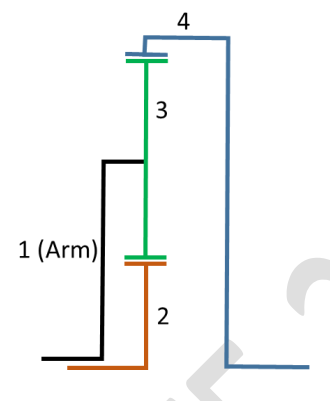
\includegraphics[width=0.35\columnwidth]{Figs/image (81).png}
\caption*{}
\label{fig:q52}
\end{figure}

\hfill{\brak{\text{GATE ME 2024}}}

\vspace{4mm}

\item
A horizontal beam of length $1200~\text{mm}$ is pinned at the left end and is resting on a roller at the other end as shown in the figure. A linearly varying distributed load is applied on the beam. The magnitude of maximum bending moment acting on the beam is \underline{\hspace{2cm}}~N.m. \brak{\text{rounded off to 1 decimal place}}.

\begin{figure}[h]
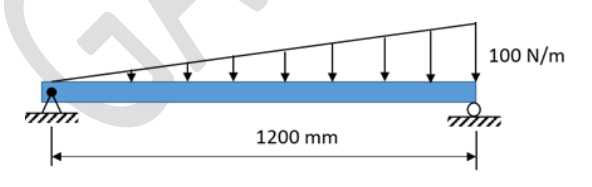
\includegraphics[width=0.46\columnwidth]{Figs/image (82).png}
\caption*{}
\label{fig:q53}
\end{figure}

\hfill{\brak{\text{GATE ME 2024}}}


\item
At the instant when OP is vertical and AP is horizontal, the link OD is rotating counter clockwise at a constant rate $\omega = 7~\text{rad/s}$. Pin P on link OD slides in the slot BC of link ABC which is hinged at A, and causes a clockwise rotation of the link ABC. The magnitude of angular velocity of link ABC for this instant is \underline{\hspace{2cm}}~rad/s \brak{\text{rounded off to 2 decimal places}}.

\begin{figure}
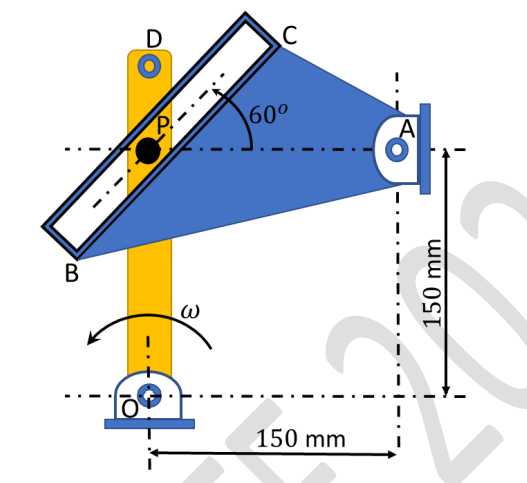
\includegraphics[width=0.48\columnwidth]{Figs/image (83).png}
\caption*{}
\label{fig:q54}
\end{figure}

\hfill{\brak{\text{GATE ME 2024}}}

\item
A vibratory system consists of mass $m$, a vertical spring of stiffness $2k$ and a horizontal spring of stiffness $k$. The end $A$ of the horizontal spring is given a horizontal motion $x_A = a\sin\omega t$. The other end of the spring is connected to an inextensible rope that passes over two massless pulleys as shown. Assume $m = 10~\text{kg}$, $k = 1.5~\text{kN/m}$, and neglect friction. The magnitude of critical driving frequency for which the oscillations of mass $m$ tend to become excessively large is \underline{\hspace{2cm}}~rad/s \brak{\text{answer in integer}}.

\begin{figure}[h]
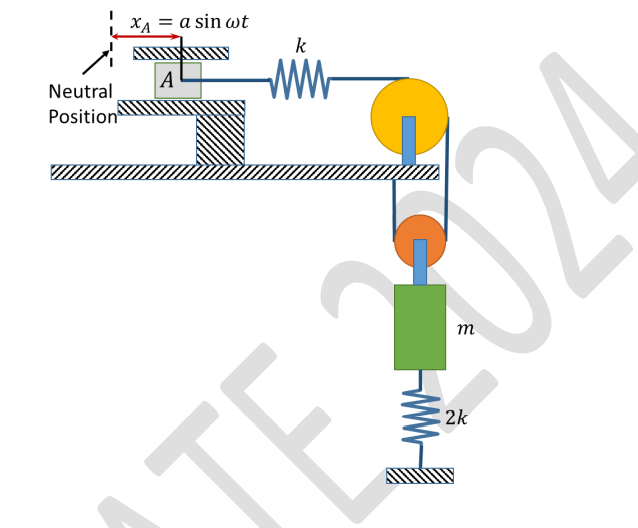
\includegraphics[width=0.54\columnwidth]{Figs/image (84).png}
\caption*{}
\label{fig:q55}
\end{figure}

\hfill{\brak{\text{GATE ME 2024}}}

\vspace{4mm}

\item
A solid massless cylindrical member of $50~\text{mm}$ diameter is rigidly attached at one end, and is subjected to an axial force $P = 100~\text{kN}$ and a torque $T = 600~\text{N}\cdot\text{m}$ at the other end as shown. Assume that the axis of the cylinder is normal to the support. Considering distortion energy theory with allowable yield stress as $300~\text{MPa}$, the factor of safety in the design is \underline{\hspace{2cm}} \brak{\text{rounded off to 1 decimal place}}.

\begin{figure}[h]
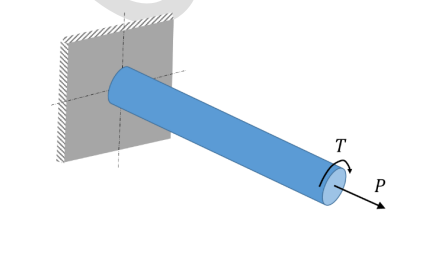
\includegraphics[width=0.37\columnwidth]{Figs/image (85).png}
\caption*{}
\label{fig:q56}
\end{figure}

\hfill{\brak{\text{GATE ME 2024}}}

\vspace{4mm}

\item
The figure shows a thin cylindrical pressure vessel constructed by welding plates together along a line that makes an angle $\alpha = 60\degree$ with the horizontal. The closed vessel has a wall thickness of $10~\text{mm}$ and diameter of $2~\text{m}$. When subjected to an internal pressure of $200~\text{kPa}$, the magnitude of the normal stress acting on the weld is \underline{\hspace{2cm}}~MPa \brak{\text{rounded off to 1 decimal place}}.

\begin{figure}[h]
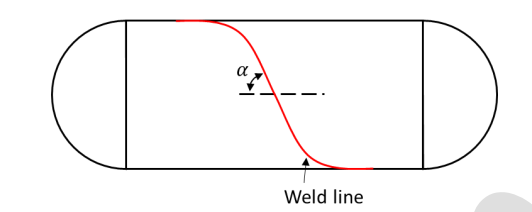
\includegraphics[width=0.48\columnwidth]{Figs/image (86).png}
\caption*{}
\label{fig:q57}
\end{figure}

\hfill{\brak{\text{GATE ME 2024}}}

\vspace{4mm}

\item
A three-hinge arch ABC in the form of a semi-circle is shown in the figure. The arch is in static equilibrium under vertical loads of $P = 100~\text{kN}$ and $Q = 50~\text{kN}$. Neglect friction at all the hinges. The magnitude of the horizontal reaction at B is \underline{\hspace{2cm}}~kN \brak{\text{rounded off to 1 decimal place}}.

\begin{figure}[h]
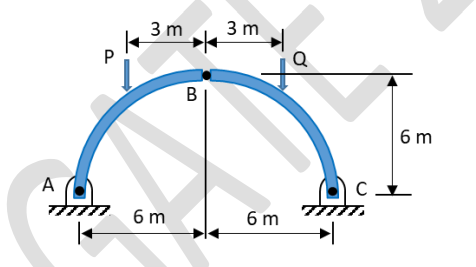
\includegraphics[width=0.50\columnwidth]{Figs/image (87).png}
\caption*{}
\label{fig:q58}
\end{figure}
\newpage
\hfill{\brak{\text{GATE ME 2024}}}

\vspace{4mm}

\item
A band brake shown in the figure has a coefficient of friction of $0.3$. The band can take a maximum force of $1.5~\text{kN}$. The maximum braking force $F$ that can be safely applied is \underline{\hspace{2cm}}~N \brak{\text{rounded off to the nearest integer}}.

\begin{figure}[h]
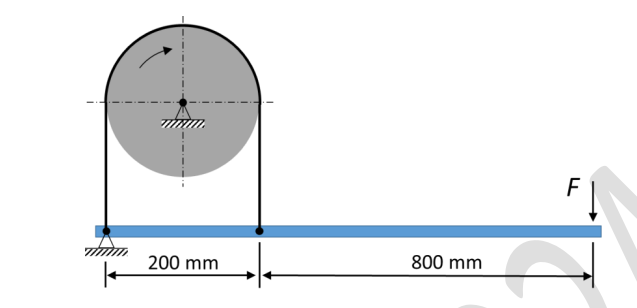
\includegraphics[width=0.56\columnwidth]{Figs/image (88).png}
\caption*{}
\label{fig:q59}
\end{figure}

\hfill{\brak{\text{GATE ME 2024}}}

\vspace{4mm}

\item
A cutting tool provides a tool life of $60$ minutes while machining with the cutting speed of $60~\text{m/min}$. When the same tool is used for machining the same material, it provides a tool life of $10$ minutes for a cutting speed of $100~\text{m/min}$. If the cutting speed is changed to $80~\text{m/min}$ for the same tool and work material combination, the tool life computed using Taylor's tool life model is \underline{\hspace{2cm}}~minutes \brak{\text{rounded off to 2 decimal places}}.

\hfill{\brak{\text{GATE ME 2024}}}

\vspace{4mm}

\item
Aluminium is casted in a cube-shaped mold having dimensions as $20~\text{mm} \times 20~\text{mm} \times 20~\text{mm}$. Another mold of the same mold material is used to cast a sphere of aluminium having a diameter of $20~\text{mm}$. The pouring temperature for both cases is the same. The ratio of the solidification times of the cube-shaped mold to the spherical mold is \underline{\hspace{2cm}} \brak{\text{answer in integer}}.

\hfill{\brak{\text{GATE ME 2024}}}

\vspace{4mm}

\item
A blanking operation is performed on C20 steel sheet to obtain a circular disc having a diameter of $20~\text{mm}$ and a thickness of $2~\text{mm}$. An allowance of $0.04$ is provided. The punch size used for the operation is \underline{\hspace{2cm}}~mm \brak{\text{rounded off to 2 decimal places}}.

\hfill{\brak{\text{GATE ME 2024}}}

\vspace{4mm}

\item
In an arc welding process, the voltage and current are $30~\text{V}$ and $200~\text{A}$, respectively. The cross-sectional area of the joint is $20~\text{mm}^2$ and the welding speed is $5~\text{mm/s}$. The heat required to melt the material is $20~\text{J/s}$. The percentage of heat lost to the surrounding during the welding process is \underline{\hspace{2cm}}~\brak{\text{rounded off to 2 decimal places}}.

\hfill{\brak{\text{GATE ME 2024}}}

\vspace{4mm}

\item
A flat surface of a C60 steel having dimensions of $100~\text{mm}$ (length) $\times$ $200~\text{mm}$ (width) is produced by a HSS slab mill cutter. The 8-toothed cutter has $100~\text{mm}$ diameter and $200~\text{mm}$ width. The feed per tooth is $0.1~\text{mm}$, cutting velocity is $20~\text{m/min}$ and depth of cut is $2~\text{mm}$. The machining time required to remove the entire stock is \underline{\hspace{2cm}}~minutes \brak{\text{rounded off to 2 decimal places}}.

\hfill{\brak{\text{GATE ME 2024}}}

\vspace{4mm}

\item
In a supplier-retailer supply chain, the demand of each retailer, the capacity of each supplier, and the unit cost in rupees of material supply from each supplier to each retailer are tabulated below. The supply chain manager wishes to minimize the total cost of transportation across the supply chain.

\begin{table}[h]
\centering
\begin{tabular}{|c|c|c|c|c|c|} \hline
         & Retailer I & Retailer II & Retailer III & Retailer IV & Capacity \\
\hline
Supplier A & 11 & 16 & 19 & 13 & 300 \\
Supplier B & 5  & 10 & 7  & 8  & 300 \\
Supplier C & 12 & 14 & 17 & 11 & 300 \\
Supplier D & 8  & 15 & 11 & 9  & 300 \\
\hline
Demand    & 300 & 300 & 300 & 300 & \\
\hline
\end{tabular}
\caption*{}
\label{tab:Q65}
\end{table}

The optimal cost of satisfying the total demand from all retailers is \underline{\hspace{2cm}}~rupees \brak{\text{answer in integer}}.

\hfill{\brak{\text{GATE ME 2024}}}


\end{enumerate}

\end{document}